\section{Diagrama de Componentes}
\label{sec:diagrama-de-componentes}

Essa seção ilustra os componentes que serão utilizados na confecção do ROV e as suas conexões por meio do diagrama da Figura \ref{fig:diagrama-de-componentes}. Nesse diagrama, as setas que conectam os componentes mostram a relação elétrica entre eles, indica se trocam informações com fio, sem fio ou somente ocorre fornecimento de energia de um componente para o outro. Os retângulos com bordas pontilhadas representam estruturas físicas do sistema. Dessa forma, nota-se que existem 10 estruturas diferentes no sistema. 

\begin{figure}[h]
	\centering
	\caption[Diagrama de Componentes]{Diagrama de Componentes}
	\label{fig:diagrama-de-componentes}
	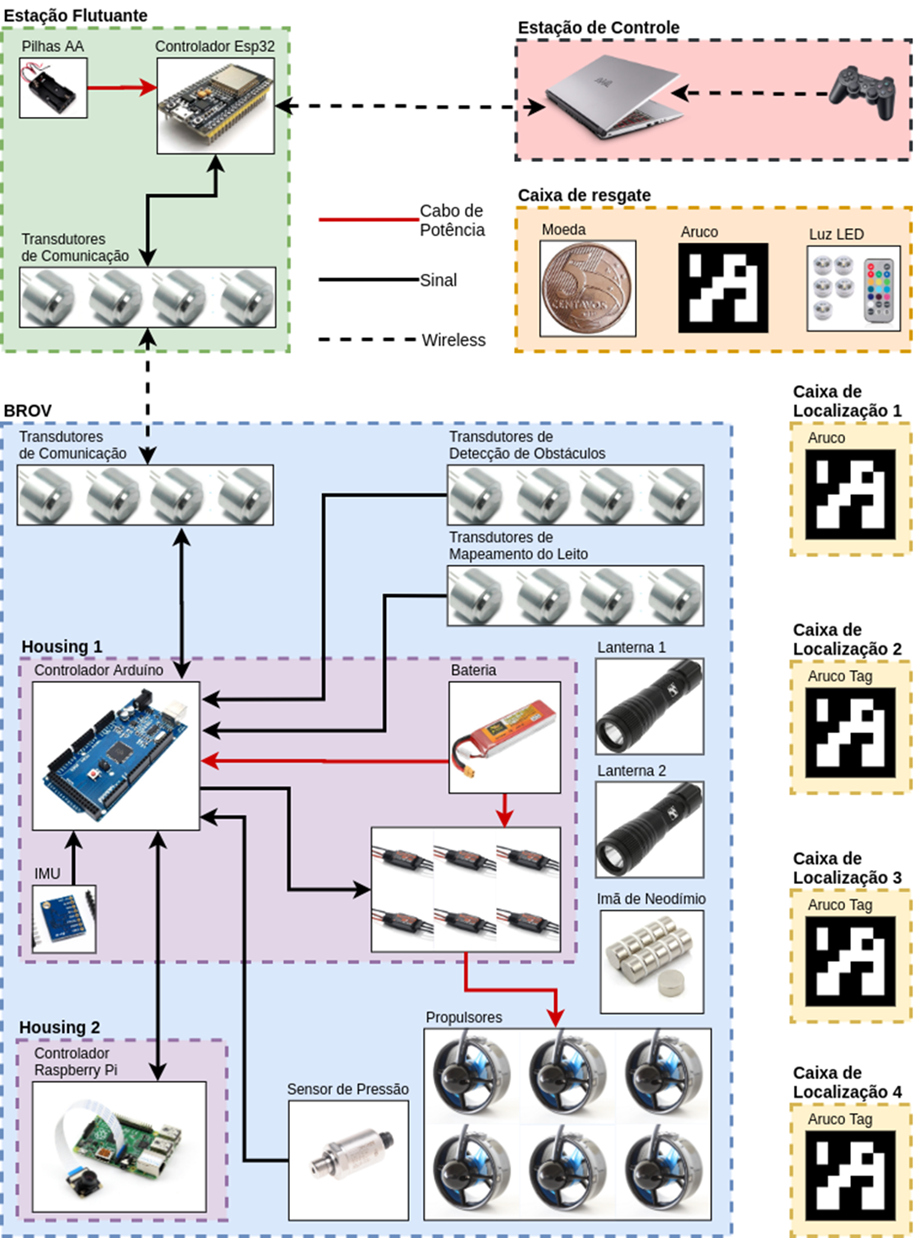
\includegraphics[width=0.9\linewidth]{images/diagrama-de-componentes}\\
	\footnotesize Fonte: Autores
\end{figure}

A estação de controle ficaria num barco, na qual se tem a possibilidade de controlar o ROV por um controle de PS3 e também por interação com a IHM presente no notebook. Essa estação apenas manda comandos para a estação flutuante e recebe dados do ROV através dessa mesma estação.

A estação de flutuante é o intermédio entre a estação de controle e o ROV, sua funcionalidade é transmitir mensagens entre essas estruturas. Nessa estação há um controlador Esp32, o qual é o responsável por converter as mensagens que chegam e enviá-las ao destinatário correto. Também estão presentes pilhas AA para alimentação do Esp32 e transdutores responsáveis por transmitir a onda ultrassom com a mensagem da estação de controle para o ROV. A troca de mensagens entre o controlador e notebook ocorre por Wi-Fi.

O ROV, representado pelo retângulo azul, tem mais duas estruturas dentro dele, duas housings, que são compartimentos vedados dentro do veículo, onde se localiza a maioria dos componentes elétricos. A housing 1 contém um Arduino mega, o qual serve somente para receber sinais de sensores e mandar comandos para os atuadores, todo o processamento é feito pelo Rapsberry Pi que está presenta na housing 2, por ter um maior poder computacional e ser compaível com a framework de programação que será usada. 

O Arduino mega recebe os sinais de três grupos de transdutores que se localizam fora da housing. Os transdutores de comunicação recebem e enviam as mensagens para a estação flutuante, como foi previamente explicado. Os transdutores de detecção de obstáculos ficam na lateral, na frente e atrás do veículo, esses servem como sensores de distâncias para identificar possíveis colisões. Os transdutores de mapeamento ficam embaixo do veículo, também funcionam como sensores de distância e tem objetivo de mapear o leito marinho. Outros sensores que ficam conectados ao Arduino são o de pressão e IMU, sendo o primeiro usado para medição de profundidade e o segundo para realização do dead-reckoning. É importante ntar que a IMU deve permanecer vedada dentro da housing 1, enquanto o sensor de pressão deve ter contato com a água.

O componente responsável pelo fornecimento de energia é a bateria de Li-Po que também fica vedada. Se escolheu utilizar essa bateria por casa do uso dos motores brushless, pelo fato de exigirem uma alta corrente, demanda-se o uso de uma bateria desse tipo. Escolheu-se esses motores pelo fato da possibilidade de se controlar sua velocidade, terem um alto rendimento e pela sua média durabilidade em meio aquoso. Para controlar a velocidade desses motores é preciso utilizar um ESC, que define a velocidade dos motores com base na PWM recebida pelo Arduino. 

Os últimos componentes na parte não vedada do ROV são as lanternas e imãs de neodímio. Os imãs vão ser utilizados em uma missão do ROV para coleta de uma moeda,a qual terá sua finalidade explicada na seção 4. Enquanto as lanternas são utilizadas para possibilitar a captura de imagem pela câmera do ROV em ambiente escuros, como o leito marinho a 10m de profundidade. A câmera fica alojada na housing 2, junto com o Raspberrry Pi, visto que tem uma conexão frágil com o controlador, precisando ficar no mesmo local para não ocorrer riscos de partir o cabo flat.

Por fim, restam as caixas com arucos, essas ficarão dispostas em um local pré definido para fornecer a localização do ROV atráves de algorítmos de visão computacinoal. A caixa de resgate, além de possuir um aruco, conta com um LED para transmissão de sinal socorro e uma moeda para coleta.
